\documentclass[11pt,a4paper]{article}
\usepackage[margin=2.3cm]{geometry}
\usepackage{amsmath,amssymb}
\usepackage{graphicx}
\usepackage{booktabs}
\usepackage{siunitx}
\usepackage{hyperref}
\usepackage{caption}
\graphicspath{{figures/}}

\newcommand{\kz}{k_z}
\newcommand{\Rt}{\tilde R}
\newcommand{\rhoMB}{\rho_{\mathrm{MB}}}

\title{Rough sea surface in the discrete nonlocal boundary condition\\
of the rational parabolic equation:\\
analytic continuation of the Miller--Brown reflection coefficient}
\author{Mikhail S.\ Lytaev}
\date{\today}

\begin{document}
\maketitle

\begin{abstract}
The discrete nonlocal boundary condition (NLBC) of the split-step Pad\'e parabolic
equation accounts for an arbitrary angle-dependent reflection coefficient of the
lower boundary, provided the coefficient admits an analytic continuation to the
complex vertical wavenumbers sampled by the inverse $z$-transform. We extend the
approach to a rough sea surface described by the Miller--Brown coherent reflection
factor. Its continuation is entire but grows off the real axis, so that $1+R$
acquires zeros inside the contour and the boundary condition becomes unstable;
no continuation that is bounded by one can reproduce the factor near grazing
incidence. Two remedies are developed: lifting the boundary to a reference plane
above the mean level, and a zero-free fitted coefficient
$1+\Rt=(1+R_f)e^{K}$ combined with a small lift. Long-range tests over ducts reveal
the conditions such a coefficient must satisfy in addition to the absence of
zeros: passivity for all propagating waves, passivity in the trapping range of
the atmosphere, and accuracy on the complex wavenumbers of range-decaying modes.
Beyond the radio horizon Miller--Brown raises the field by tens of decibels. An
independent modal and branch-cut solution shows that this is the lateral wave
that the model itself produces at grazing incidence, because its effective surface
impedance is odd in the vertical wavenumber; it is not an artefact of the boundary
condition. It contradicts the grazing behaviour established by Barrick, that the
roughness-modified impedance of any rough surface tends to a constant. We therefore
add a constant grazing impedance: the roughness admittance of Miller--Brown is kept
above a blend angle and frozen below it, evenly in the vertical wavenumber. With the
fitted coefficient matched to first order at grazing, the parabolic equation
reproduces the creeping-mode attenuation of this impedance to \SI{0.01}{dB/km}, and the
beyond-horizon excess disappears, except where the blend angle falls inside the
range of the creeping modes (X band, \SI{15}{m/s}), where it is reduced from 40 to
\SI{11}{dB}. The method agrees with an exact plane-wave-spectrum
solution to 0.1--1.2\,\% and is demonstrated for L, S and X band, wind speeds up to
\SI{15}{m/s} and three refractivity profiles over \SI{60}{km}.
\end{abstract}

%=====================================================================
\section{Introduction}

The parabolic equation (PE) is the standard tool for tropospheric radio-wave
propagation over the sea. The surface enters through the lower boundary
condition. The usual Leontovich impedance condition assumes a grazing-angle
independent impedance, and the split-step Fourier method with the mixed Fourier
transform inherits this restriction. In \cite{lytaev2022} it was shown that the
discrete nonlocal boundary condition (NLBC) of the finite-difference split-step
Pad\'e PE accommodates an \emph{arbitrary} Fresnel reflection coefficient
$R(\kz)$, including the Brewster-angle zero of vertical polarisation. The
condition is that $R$ admits an analytic continuation to the complex vertical
wavenumbers sampled by the inverse $z$-transform. The conclusion of
\cite{lytaev2022} named the Miller--Brown rough-surface model \cite{mbv1984} as a
natural next step and identified the analytic continuation as the open problem.
Miller--Brown is the coherent reflection model most widely used with
split-step Fourier PE codes; its accuracy for forward propagation was assessed
numerically in \cite{freund2006}.

\paragraph{Related work.}
Barrick \cite{barrick1998} criticised the use of Miller--Brown in split-step codes:
the resulting impedance and admittance depend strongly on the grazing angle,
whereas exact modal solutions give a roughness-modified impedance that tends to a
constant at grazing, for both polarisations and any roughness. Perturbation theory
\cite{barrick1971} and the Dyson-equation treatment of the coherent field
\cite{ishimaru2000} lead to the same structure, an effective impedance equal to the
smooth one plus a roughness term, and the constant has been extracted numerically
from fields computed over rough surfaces \cite{lai2004}. Shadowing corrections to the
Ament and Miller--Brown factors reduce the effective roughness near grazing
\cite{fabbro2006,song2024,zhao2025}. The small-slope approximation
\cite{voronovich1994} covers the Kirchhoff and Bragg regimes in one theory but loses
validity once the grazing angle falls below the rms slope. A different route
avoids a reflection model altogether: random sea surfaces generated from a wave
spectrum (Pierson--Moskowitz \cite{pm1964}, JONSWAP \cite{hasselmann1973}, or
Elfouhaily \cite{elfouhaily1997}, which uses JONSWAP for the long waves) are
propagated over as terrain and averaged \cite{gao2019,guo2020,ji2025}, or the
spectrum is split, its long waves forming the geometry and its short waves a
roughness coefficient \cite{bonnafont2024}.

This report addresses that problem. Section~\ref{sec:nlbc} recalls the NLBC and the
roughness models. Section~\ref{sec:continuation} shows why the plain continuation
fails and why no bounded continuation can be exact. Section~\ref{sec:methods}
develops a lifted reference plane and a zero-free fitted coefficient, together with
the stability conditions found on long-range problems. Section~\ref{sec:lateral}
analyses the field beyond the radio horizon, and Section~\ref{sec:barrick} replaces the
grazing extrapolation of Miller--Brown by a constant impedance. Validation and a
long-range demonstration follow in Section~\ref{sec:results}.

%=====================================================================
\section{Nonlocal boundary condition and rough-surface reflection}\label{sec:nlbc}

The reduced field $u=\psi e^{-ikx}$ of the two-dimensional Helmholtz equation is
marched in range by a rational (Pad\'e) approximation of the one-way propagator,
\begin{equation}
  u^{n+1}=\prod_{l=1}^{p}\frac{1+a_l L}{1+b_l L}\,u^{n},\qquad
  L=\frac{1}{k^2}\frac{\partial^2}{\partial z^2}+\left(m^2-1\right),
\end{equation}
each factor being solved by a fourth-order Numerov scheme in $z$ \cite{collins1993,lytaev2022}.
Near the lower boundary the medium is homogeneous and the discrete vertical
equation has solutions $\mu^{\pm j}$, $|\mu|<1$, with $\kz=\log\mu/(i\Delta z)$.
A reflecting surface relates the down- and up-going parts by $R(\kz)$, giving the
$z$-transformed boundary relation
\begin{equation}
  \frac{\chi_1}{\chi_0}=\mu+\frac{\mu^{-1}-\mu}{1+R(\kz)},
\end{equation}
evaluated for each eigenvalue of the Pad\'e pencil. The convolution coefficients
$D_m$ of the NLBC follow from an inverse $z$-transform on the circle
$|\xi|=\tau>1$, computed by adaptive Filon--Clenshaw--Curtis quadrature.

\paragraph{Roughness models.}
With $x=2(\sigma\kz)^2$, $\sigma$ the rms wave height, the coherent reflection
coefficient about the mean level is $R=R_f\,\rho$, where $R_f$ is the Fresnel
coefficient and
\begin{equation}
  \rhoMB=e^{-x}I_0(x)\quad\text{(Miller--Brown \cite{mbv1984})},\qquad
  \rho_{\mathrm A}=e^{-x}\quad\text{(Ament \cite{ament1953})}.
\end{equation}
For a fully developed sea $\sigma=0.0051\,U^2$ ($U$ the wind speed in m/s) \cite{levy2000}.

%=====================================================================
\section{The analytic-continuation problem}\label{sec:continuation}

\paragraph{Where $R$ is sampled.}
The circle $|\xi|=\tau$ maps onto a closed loop in the first quadrant of the
$\kz$ plane (Fig.~\ref{fig:loop}). It runs along the real (propagating) axis, up
the imaginary (evanescent) axis and back along an arc; its interior is the image of
$|\xi|>\tau$. The boundary ratio is analytic there, and the $D_m$ are causal and
stable, if and only if $R$ is analytic inside the loop and $1+R$ has no zeros there.

\paragraph{Failure of the plain continuation.}
Both roughness factors are entire functions of $\kz$, but they grow like
$e^{4(\sigma\,\mathrm{Im}\,\kz)^2}$ off the real axis. For the H-polarised sea,
$R_f\approx-1$ and the zeros of $1+R$ are close to those of $1-\rhoMB(x)$: the first
lies at $|x|\approx3.5$, $\arg x\approx\ang{102}$, i.e.\ at $|\kz|\approx1.32/\sigma$,
$\arg\kz\approx\ang{51}$. It falls inside the loop for any appreciable roughness
(for $\sigma=\SI{0.3}{m}$ at \SI{3}{GHz} the first zeros are at
$\kz\approx2.78+3.42i$, and the loop reaches $|\kz|\approx22$). The resulting
boundary condition is wrong: the field error against the exact solution of
Section~\ref{sec:results} is 45\,\% for $\sigma=\SI{0.3}{m}$, H-pol.

\paragraph{No exact bounded continuation.}
A coefficient $\Rt$ that is analytic and bounded by one inside the loop cannot equal
$R_f\rhoMB$ on a segment of the real axis. By the identity theorem it would coincide
with the entire continuation, which is unbounded. Approximation does not escape
either: requiring $|\tilde\rho|\le1$ on the evanescent axis, where the continuation
$\rhoMB(-|x|)=e^{|x|}I_0(|x|)$ exceeds one, forces a jump in the argument of the
boundary data at $x=0$. Its harmonic conjugate is a phase of order
$(x/\pi)\log(1/x)$ near grazing (a Kramers--Kronig constraint). Numerically, the
best bounded approximation of $\rhoMB$ carries 2--18$^\circ$ of phase.

\begin{figure}[t]
  \centering
  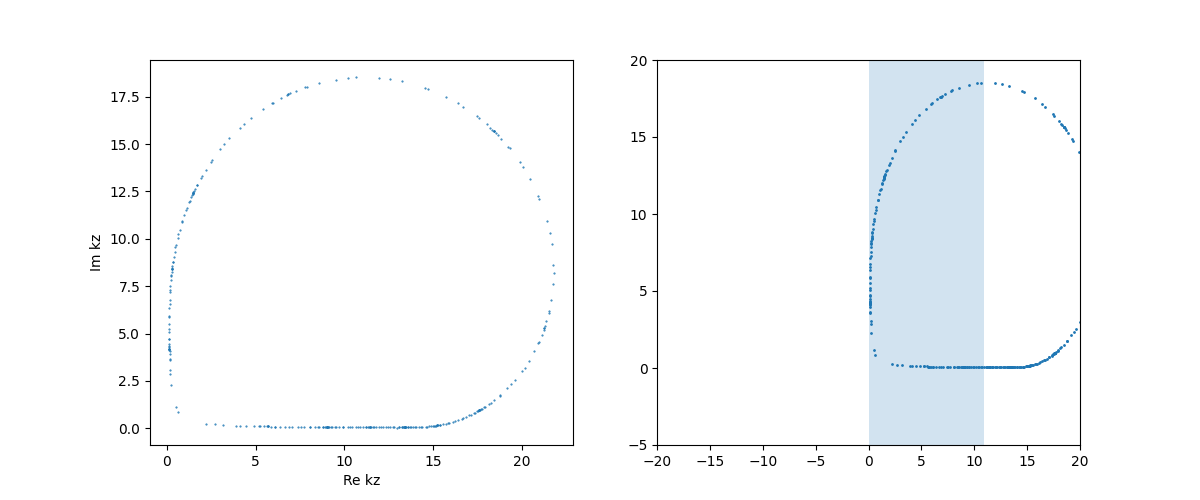
\includegraphics[width=0.75\linewidth]{kz_contour.png}
  \caption{Vertical wavenumbers sampled by the inverse $z$-transform at the lower
  boundary (\SI{3}{GHz}, Pad\'e [5/6]). Right: zoom near the origin; shaded: the
  propagating range $[0,k_{z,\max}]$.}
  \label{fig:loop}
\end{figure}

%=====================================================================
\section{Remedies}\label{sec:methods}

\subsection{Reference plane above the mean level}
A boundary condition can only represent scatterers below it, while the wave crests
rise above the mean level. Placing the boundary at height $z_0$ and re-referencing
the reflection coefficient,
\begin{equation}
  R_{z_0}(\kz)=R_f(\kz)\,\rho(\kz)\,e^{2i\kz z_0},
\end{equation}
reproduces the mean-level rough reflection exactly at every real grazing angle
(a pure reference-plane phase), while $|e^{2i\kz z_0}|=e^{-2z_0\,\mathrm{Im}\,\kz}$
damps the growth. The smallest admissible lift follows from the maximum-modulus
principle: if $|R_{z_0}|\le1$ on the loop, then $|R_{z_0}|<1$ inside it, and $1+R$
cannot vanish. Since $\log|R_{z_0}|$ is linear in $z_0$ at every contour point,
\begin{equation}
  z_0=\max_{\text{loop}}\frac{\log|R_f\rho|}{2\,\mathrm{Im}\,\kz}.
\end{equation}
The method is exact but $z_0$ grows like $\sigma^2$ times the loop size:
\SI{2.6}{m} for $\sigma=\SI{0.3}{m}$ at \SI{3}{GHz}, but \SI{11}{m} and \SI{78}{m} for
X band at 10 and \SI{15}{m/s}. The field below $z_0$ is not computed, and a large
lift removes refracting air below the plane.

\subsection{Zero-free fitted coefficient}
The stability condition does not require $|\Rt|\le1$, only that $1+\Rt$ have no
zeros. This is built in by
\begin{equation}
  1+\Rt(\kz)=\bigl(1+R_f(\kz)\bigr)\,e^{K(\kz)},
\end{equation}
since $1+R_f$ is zero-free (the smooth condition is stable) for \emph{any} analytic
$K$. $K$ is fitted by least squares to $\log\bigl[(1+R)/(1+R_f)\bigr]$:
\begin{itemize}
\item \emph{Basis.} A polynomial in $\kz$ of degree 40 (80 if needed), with the
  Vandermonde-with-Arnoldi orthogonalisation \cite{brubeck2021}. When a lift is
  used, $\log(1+R_{z_0})$ is a power series in the lift phase, so
  $K=\sum_{n\le6}e^{2in\kz z_0}P_n(\kz)$. Each harmonic is bounded by one in the
  upper half plane.
\item \emph{Accuracy} on the propagating range $[0,1.2\,k_{z,\max}]$, measured as the
  relative error of $1+R$. Near grazing $R\to-1$, and an absolute error in $R$
  would misplace the effective surface impedance.
\item \emph{Regularisation.} A Tikhonov term on the loop is relaxed until the
  tolerance ($5\times10^{-3}$) is met, keeping $|\mathrm{Re}\,K|\le15$. The loop is
  thinned on a spatial grid: it holds tens of thousands of nearly coincident
  samples, and a stride aliases with their ordering.
\end{itemize}
For strong roughness the zeros of the continued $1+R$ approach the propagating
range and no moderate $K$ fits. The boundary is then lifted by the smallest $z_0$
(in fractions of $\sigma$) that makes the fit admissible. In all cases studied
this is a few centimetres to \SI{1.7}{m}, compared with up to \SI{78}{m} for the pure lift.

\subsection{Stability conditions found on long-range problems}
Zero-freeness proved necessary but not sufficient. Each of the following
conditions was found from a failure on a long-range problem, and each is now part of
the admissibility test of a fit:
\begin{enumerate}
\item \emph{Passivity for propagating waves:} $|\Rt|\le1$ on the whole real stretch of
  the loop, not only on the fitted range. Otherwise a propagating wave gains energy
  at every bounce and diverges in a duct (L band, \SI{15}{m/s}, evaporation duct).
\item \emph{Passivity in the trapping range:} $|\Rt|\le1$ in the quarter disc
  $|\kz|\le k\sqrt{2\cdot10^{-6}\Delta M}$ above the real axis, where $\Delta M$ is the
  modified-refractivity deficit of a trapping layer. A layer returns these waves to
  the surface, and an active surface would resonate with it (X band, \SI{15}{m/s}).
\item \emph{Accuracy for range-decaying modes:} the creeping modes beyond the horizon
  sit at $\arg\kz\approx-\ang{60}$, $|\kz|=\sqrt{|a_n|}\,(k^2g)^{1/3}$ with $a_n$ the Airy
  zeros and $g=\mathrm{d}m^2/\mathrm{d}z$. Trapped duct modes lie just below the real
  axis. $K$ is fitted to the continued $R$ on these sectors as well; otherwise the
  polynomial is unconstrained there. With the sectors included, the creeping-mode
  attenuations computed with $\Rt$ agree with those of the exact Miller--Brown
  coefficient to \SI{0.01}{dB/km}.
\item \emph{First-order accuracy at grazing:} $K$ is matched to the value and the
  slope of its target at $\kz=0$ (central differences across the origin, as
  heavily weighted rows of the least-squares problem). Since $1+R_f=O(\kz)$, then
  $\Rt-R=O(\kz^3)$ and the effective impedance (Section~\ref{sec:lateral}) is exact
  to $O(\kz^2)$: the fit adds no odd linear term to it. Without this condition a
  residual slope of $K$ of order $10^{-3}$, harmless for Miller--Brown, left a
  lateral wave some \SI{20}{dB} below that of Miller--Brown when the grazing
  impedance is small (Section~\ref{sec:barrick}). With it, the odd part of the fitted
  impedance near grazing drops from $10^{-5}$ to $10^{-10}$ of its value.
\end{enumerate}

%=====================================================================
\section{The field beyond the radio horizon}\label{sec:lateral}

Over a rough sea described by Miller--Brown the computed field far beyond the
horizon in a standard atmosphere exceeds the smooth-sea field by tens of decibels
at 10--\SI{15}{m/s}. It is nearly uniform in height and decays slowly with range. An
independent solution of the continuous problem shows that this is a property of
the roughness model, not of the boundary condition. We found no support for it in
other studies: PE computations with shadowed roughness factors or explicit rough
surfaces report propagation loss that increases with wind speed
\cite{gao2019,song2024}, and the effective impedance of a rough surface is constant
at grazing \cite{barrick1998}, whereas that of Miller--Brown is not.

\paragraph{Independent solution.}
In the earth-flattened standard atmosphere $m^2=1+gz$, the vertical solutions are
Airy functions. The line-source Green's function is
\begin{equation}
  G(x,z)=\frac{1}{2\pi}\int g(z,z_s;k_x)\,e^{ik_xx}\,dk_x,
\end{equation}
with $g=\phi_b(z_<)\phi_{\mathrm{out}}(z_>)/W$. Here
$\phi_{\mathrm{out}}=\mathrm{Ai}(s)-i\,\mathrm{Bi}(s)$ radiates upward, and $\phi_b$
satisfies the impedance condition $u'/u=i\kappa$ with
\begin{equation}
  \kappa(\kz)=\kz\,\frac{R(\kz)-1}{R(\kz)+1}.
\end{equation}
Deforming the contour for large $x$ gives the residues at the creeping modes plus
an integral along the branch cut at $k_x=k$ ($\kz=0$). The two sides of the cut
correspond to $\pm\kz$, and the cut integral (the lateral wave) is driven by the
odd part of $\kappa$. For the smooth sea (H-pol) $\kappa=-q$,
$q=k\sqrt{\varepsilon-1+\kz^2/k^2}$, is even: no lateral wave, and the field decays
exponentially (\SI{2.41}{dB/km} at X band, against \SI{2.50}{dB/km} from the PE).
With Miller--Brown, near grazing
\begin{equation}
  \kappa\approx-\frac{q}{1+q\sigma^2\kz},
\end{equation}
which is odd in $\kz$. The model itself predicts a lateral wave. More generally,
$\kappa$ of $R=R_f\rho$ is even if and only if $\rho(\kz)\rho(-\kz)=1$, which an even
roughness factor violates. (With the down-going wave $e^{-i\kz z}+Re^{i\kz z}$ the
condition reads $u_z=i\kappa u$; real negative $\kappa$ is absorbing.)

Figure~\ref{fig:impedance} shows $|\kappa|$ against the grazing angle. For the
smooth sea it is constant. With Miller--Brown or Ament at H polarisation it falls
roughly as $1/\kz$ over two decades of angle and has not reached the smooth value
even at \ang{0.001} at \SI{15}{m/s}; the constant region of the model,
$\kz\ll1/(q\sigma^2)$, lies below \SI{e-4}{rad} at \SI{3}{GHz} and \SI{10}{m/s}. Ament
with Smith shadowing moves the transition to angles about ten times smaller but
does not remove it. At V polarisation all models stay near the smooth value below
about \ang{0.05}, in line with Barrick's observation that Miller--Brown is roughly
adequate for VV but not for HH \cite{barrick1998}.

\begin{figure}[t]
  \centering
  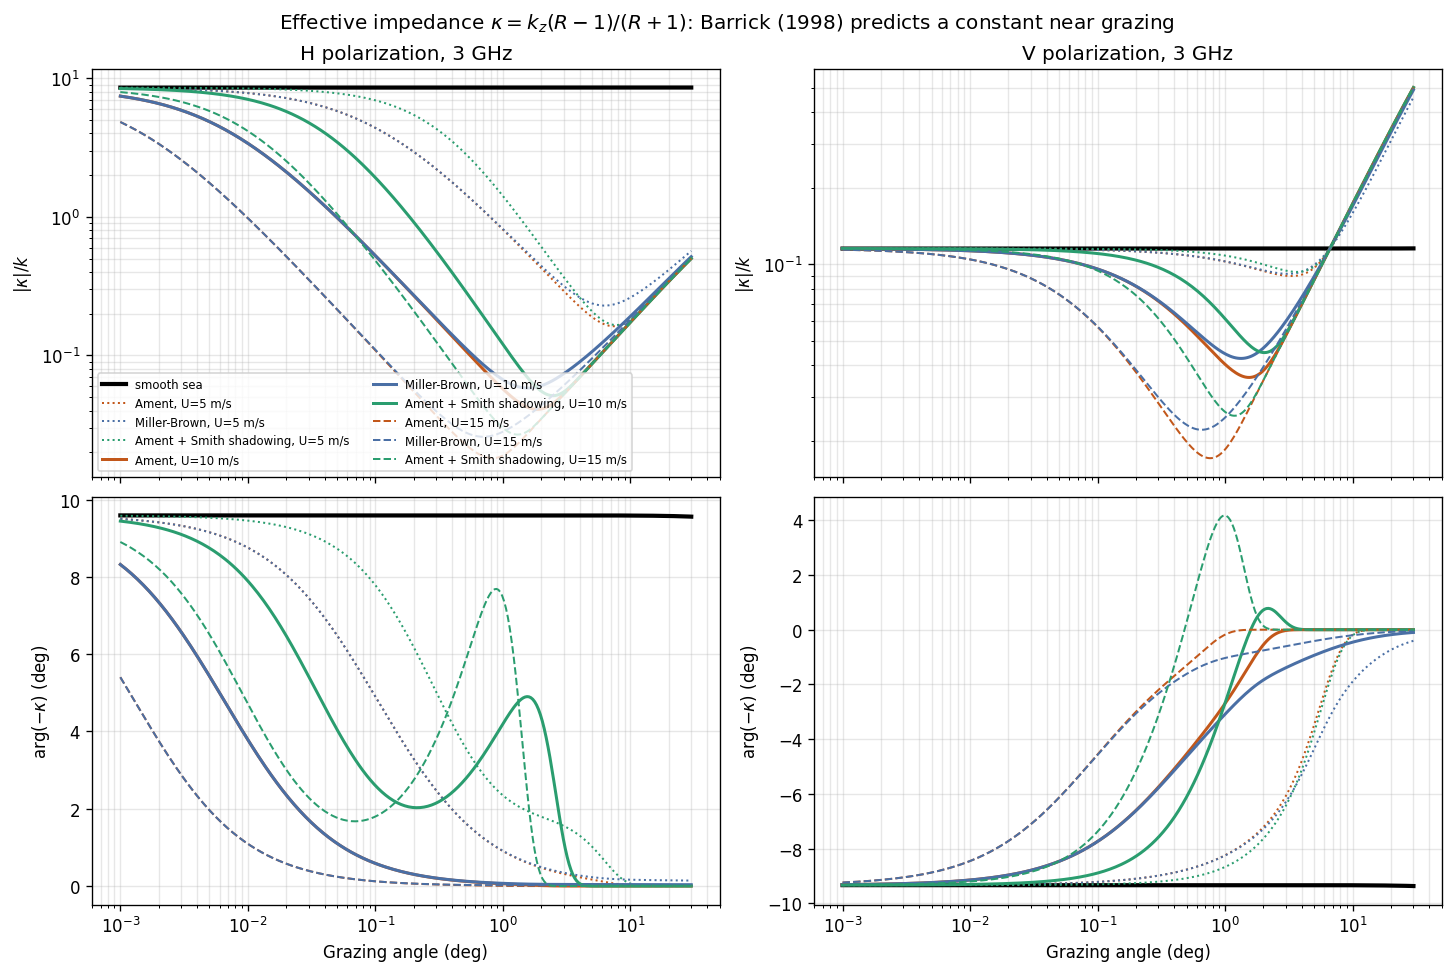
\includegraphics[width=\linewidth]{rough_sea_impedance_angle.png}
  \caption{Effective impedance $\kappa=\kz(R-1)/(R+1)$ against the grazing angle,
  \SI{3}{GHz}, $\varepsilon=70$, \SI{4}{S/m}, $\sigma=0.0051U^2$; the Smith shadowing
  uses the Cox--Munk upwind slope. Top: $|\kappa|/k$; bottom: $\arg(-\kappa)$.}
  \label{fig:impedance}
\end{figure}

\paragraph{Comparison.}
Table~\ref{tab:lateral} compares the excess field over the smooth sea at
\SI{58}{km}, \SI{10}{m} height. The PE with the fitted coefficient follows the
independent Miller--Brown solution at \SI{10}{m/s} and above. At \SI{5}{m/s}, deep
in the shadow (path loss about \SI{235}{dB}), it differs by about \SI{11}{dB}: the
continued impedance has a singularity at $\kz=-1/(q\sigma^2)$, close to the
origin, which a polynomial $K$ cannot represent. The lateral wave samples $R$ on
that side of the cut.

\begin{table}[t]
  \centering
  \caption{Field relative to the smooth sea (dB) beyond the horizon, X band,
  standard atmosphere, antenna at \SI{20}{m}, \SI{58}{km} range, \SI{10}{m} height.}
  \label{tab:lateral}
  \begin{tabular}{lccc}
    \toprule
    Wind speed & Independent, exact MB & Independent, MB at $z_0=3\sigma$ & PE, fitted $\Rt$ \\
    \midrule
    \SI{5}{m/s}  & $-4.2$  & $+2.5$  & $+7.0$ \\
    \SI{10}{m/s} & $+26.2$ & $+26.0$ & $+26.4$ \\
    \SI{15}{m/s} & $+40.6$ & $+38.1$ & $+39.7$ \\
    \bottomrule
  \end{tabular}
\end{table}

\paragraph{What does not remove it.}
Lifting the reference plane leaves the excess essentially unchanged (Table~\ref{tab:lateral}),
because the lift factor $e^{2i\kz z_0}$ is itself odd across the cut. A passive
roughness factor $|\tilde\rho|\le1$, built as the Schwarz integral of
$\log|\tilde\rho|=\log\rhoMB$ on the propagating axis, introduces an
$x\log x$ branch point at grazing. That again creates a lateral wave, and unless
$\tilde\rho(0)=1$ is enforced exactly, it also moves the trivial grazing root of the
mode equation off zero into a lossless mode. Finally, an exactly
lateral-wave-free factor $\tilde\rho=e^{\kz H(\kz^2)}$ cannot follow the quadratic
onset of $\rhoMB$ without square-root behaviour on the evanescent axis, inside the
contour. Within the Miller--Brown model the lateral wave could only be removed by
switching roughness off at grazing angles up to about \ang{0.16} at X band, which
are exactly the angles that matter for ducting. The beyond-horizon excess is
therefore a consequence of extrapolating Miller--Brown to grazing angles of order
$10^{-5}$\,rad. The next section keeps the roughness at these angles but replaces
the extrapolation by a constant impedance.

%=====================================================================
\section{Constant grazing impedance}\label{sec:barrick}

\paragraph{Blend.}
In terms of the admittance $Y=1/\kappa=(R+1)/\bigl(\kz(R-1)\bigr)$, the roughness
adds $Y_r=Y-Y_f$ to the smooth-sea admittance $Y_f$; near grazing Miller--Brown
gives $Y_r\approx-\sigma^2\kz$, the odd term of the previous section. We replace it by
\begin{equation}
  Y_B(\kz)=Y_f(\kz)+Y_r\!\left(\sqrt{\kz^2+k_g^2}\right),\qquad
  R_B=\frac{\kz Y_B+1}{\kz Y_B-1},
\end{equation}
where $Y_r$ is evaluated with the exact Miller--Brown coefficient. $Y_f$ and the
argument of $Y_r$ are even in $\kz$, so the impedance is even and there is no
roughness-induced lateral wave. Below $k_g$ the impedance is constant,
$\kappa_g=1/\bigl(Y_f(0)+Y_r(k_g)\bigr)$, as required by \cite{barrick1998}; well
above $k_g$ the blend coincides with Miller--Brown. $R_B(0)=-1$, and
$|R_B|\le1$ on the real axis (checked numerically for 1--\SI{10}{GHz} and
5--\SI{15}{m/s}). The square root has branch points at $\kz=\pm ik_g$, so the
blend is used with the zero-free fit only, which samples $R$ on the real axis and
on the sectors below it.

\paragraph{Blend angle.}
We place $k_g=1/(2\sigma)$, where the Rayleigh roughness parameter $2\kz\sigma$
reaches one: Kirchhoff (Miller--Brown) above, effective impedance below. This is
\ang{0.89} at \SI{3}{GHz} and \SI{10}{m/s} and \ang{0.40} at \SI{15}{m/s}. For strong
roughness $\kappa_g\approx-2/\sigma$, nearly real: $\kappa_g/k=-0.072$ at
\SI{3}{GHz} and \SI{10}{m/s}, against $|\kappa|/k=8.6$ for the smooth sea. The constant
is a heuristic. Barrick's theory fixes that the impedance is constant, not its value.
A self-consistent choice $k_g=|\kappa_g|$ (the constant region ending at the
pseudo-Brewster angle) has no solution at H polarisation, where the whole angular
range satisfies $\sin\psi<|\kappa|/k$, and at V polarisation returns the smooth-sea
pseudo-Brewster angle. A calibrated value requires rigorous solutions over
spectrum-generated sea surfaces, by the method of moments \cite{freund2006} or
Monte Carlo PE \cite{gao2019}.

\paragraph{Check against the modes.}
Beyond the horizon the field of a constant impedance is a sum of creeping modes
with no cut contribution. With $u=\mathrm{Ai}\bigl(\omega(-z/\ell-t)\bigr)$,
$\omega=e^{2\pi i/3}$, $\ell=(k^2g)^{-1/3}$, the condition $u_z=i\kappa u$ gives
$\mathrm{Ai}(s)+\omega\,\mathrm{Ai}'(s)/(i\kappa\ell)=0$ with $s=-\omega t$, and the mode
attenuation is $-\mathrm{Im}\,t/(2k\ell^2)$. For the blend the same equation is solved
with $\kappa(\kz)$, $\kz=\sqrt t/\ell$. Table~\ref{tab:modes} compares the first-mode
attenuation with the range slope of the PE path loss at \SI{10}{m} over
45--\SI{58}{km}, less \SI{0.084}{dB/km} of cylindrical spreading.

\begin{table}[t]
  \centering
  \caption{Beyond-horizon decay (dB/km) in the standard atmosphere: PE slope at
  \SI{10}{m}, 45--\SI{58}{km}, against the first creeping mode of the same boundary
  condition; last column: rough minus smooth path loss at \SI{58}{km}. Antenna
  at \SI{20}{m}, H-pol.}
  \label{tab:modes}
  \begin{tabular}{llccc}
    \toprule
    Band & Surface & PE & Mode 1 & Excess loss (dB) \\
    \midrule
    S & smooth & 1.613 & 1.615 & -- \\
      & Miller--Brown, \SI{10}{m/s} & 1.844 & 1.613 & $+2.7$ \\
      & Miller--Brown, \SI{15}{m/s} & 0.048 & 1.605 & $-8.7$ \\
      & blend, \SI{10}{m/s} & 1.595 & 1.596 & $-0.7$ \\
      & blend, \SI{15}{m/s} & 1.566 & 1.573 & $-1.8$ \\
    \midrule
    X & smooth & 2.413 & 2.412 & -- \\
      & Miller--Brown, \SI{10}{m/s} & $-0.020$ & 2.398 & $-26.4$ \\
      & Miller--Brown, \SI{15}{m/s} & 0.388 & 2.332 & $-39.7$ \\
      & blend, \SI{10}{m/s} & 2.357 & 2.351 & $-2.4$ \\
      & blend, \SI{15}{m/s} & 1.913 & 2.278 & $-11.3$ \\
      & constant $\kappa_g$, \SI{15}{m/s} & 2.274 & 2.271 & $-5.1$ \\
    \bottomrule
  \end{tabular}
\end{table}

The PE follows the modes of the blend to \SI{0.01}{dB/km} at S band and at X band,
\SI{10}{m/s}; the Miller--Brown runs do not, because the lateral wave dominates. The
rough-sea field then stays within a few decibels of the smooth one: the small,
nearly real $\kappa_g$ makes the surface less Dirichlet-like than the smooth sea and
lowers the creeping-mode attenuation by 0.02--\SI{0.13}{dB/km}. At X band and
\SI{15}{m/s} the blend angle lies inside the creeping-mode range,
$k_g=0.44<3(k^2g)^{1/3}=\SI{0.72}{m^{-1}}$. The modes then sample the transition of
the blend and its branch point, and the far field depends on the blend shape: the
slope is \SI{1.91}{dB/km} with the Rayleigh $k_g$, \SI{2.18}{dB/km} with
$k_g=1/\sigma$, and \SI{2.27}{dB/km} for a constant $\kappa_g$ at all angles, which
again matches its mode. The implementation warns in this case. In the
\SI{15}{m} evaporation duct at S band both models change the loss at \SI{10}{m} by
less than \SI{1.5}{dB} over \SI{60}{km} (Fig.~\ref{fig:blend}).

\begin{figure}[t]
  \centering
  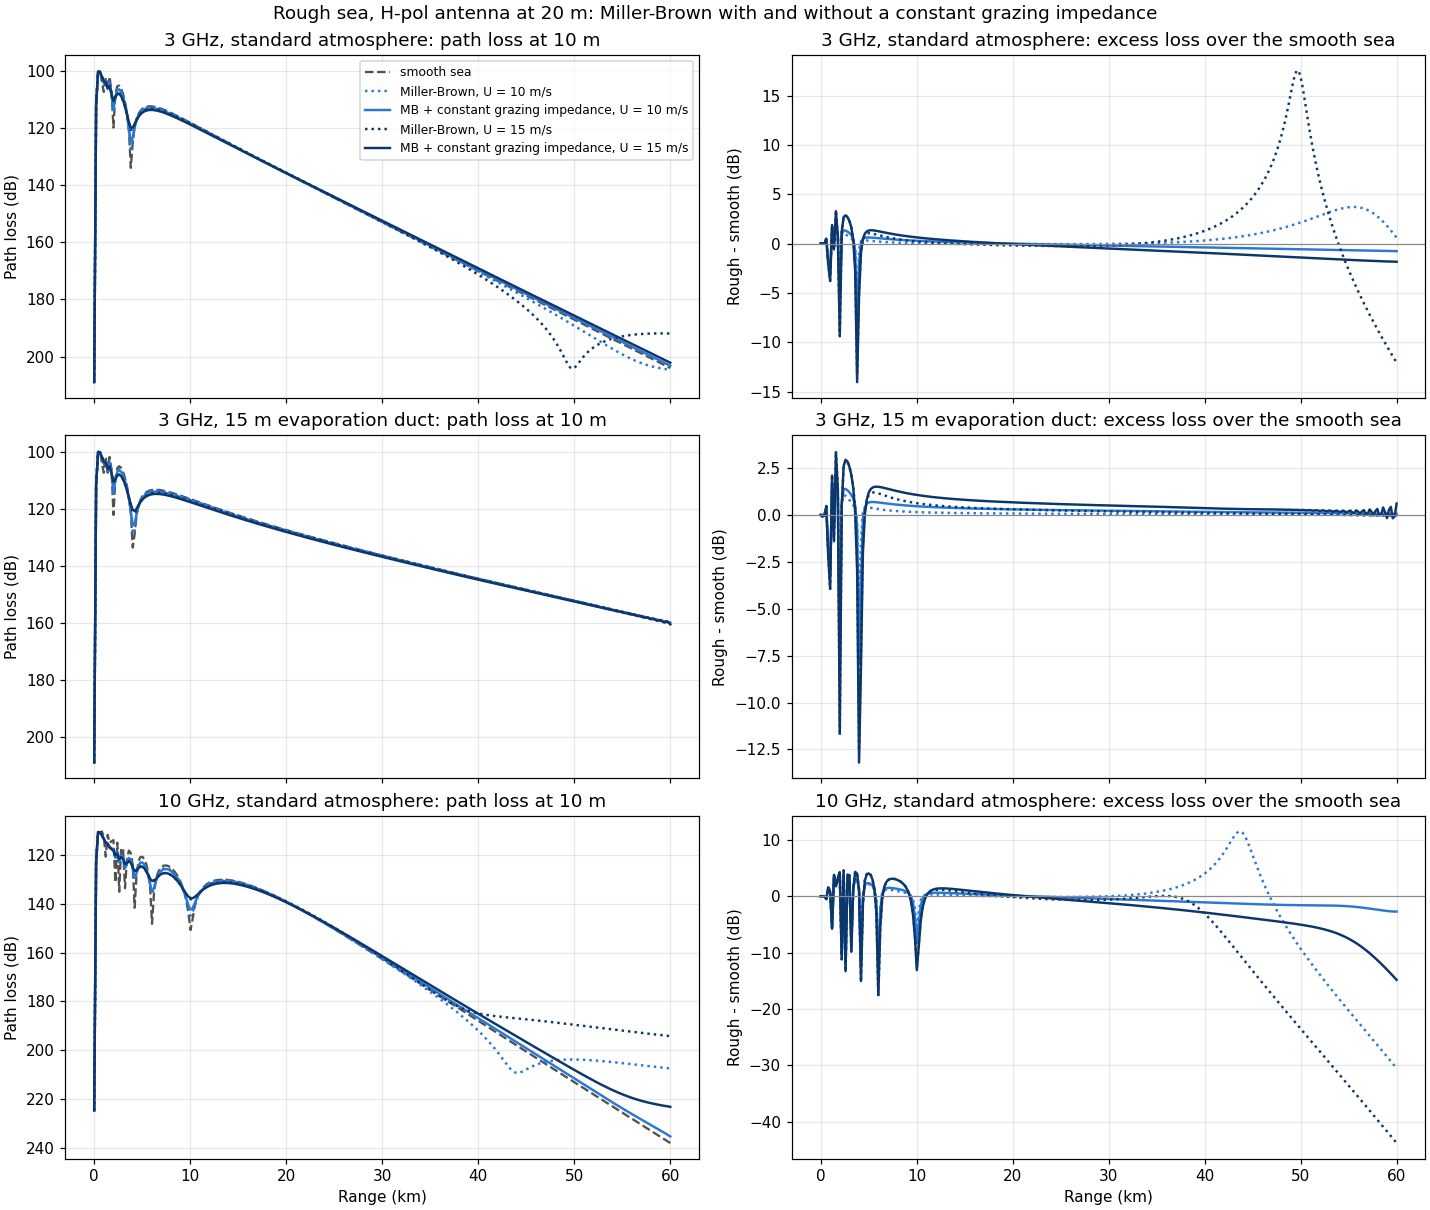
\includegraphics[width=\linewidth]{rough_sea_grazing_blend_demo.png}
  \caption{Path loss at \SI{10}{m} (left) and excess over the smooth sea (right):
  Miller--Brown (dotted) and Miller--Brown with the constant grazing impedance
  (solid), 10 and \SI{15}{m/s}. Rows: S band in a standard atmosphere and in a
  \SI{15}{m} evaporation duct, X band in a standard atmosphere.}
  \label{fig:blend}
\end{figure}

%=====================================================================
\section{Results}\label{sec:results}

\subsection{Validation against an exact solution}
For a Gaussian beam over a flat surface in a homogeneous medium the one-way field
is the plane-wave spectrum of the source, each down-going component reflected with
$R(|\kz|)$. Table~\ref{tab:validation} lists the relative error of $|u|$ beyond the
specular point. Short-range cases use \SI{3}{GHz}, a 30\,m antenna and
\ang{5} elevation; X band cases use \SI{5}{km}, a 20\,m antenna and \ang{0.5}
elevation. The smooth-sea error is 0.6\,\%.

\begin{table}[t]
  \centering
  \caption{Relative error of $|u|$ against the exact solution, zero-free fit.}
  \label{tab:validation}
  \begin{tabular}{llccc}
    \toprule
    Frequency & $\sigma$ & Lift $z_0$ & H-pol & V-pol \\
    \midrule
    \SI{3}{GHz}  & \SI{0.1}{m}  & 0--\SI{0.01}{m} & 0.8\,\% & 1.2\,\% \\
    \SI{3}{GHz}  & \SI{0.3}{m}  & 0--\SI{0.03}{m} & 1.1\,\% & 1.1\,\% \\
    \SI{10}{GHz} & \SI{0.51}{m} & \SI{0.10}{m} & 0.08\,\% & 0.15\,\% \\
    \SI{10}{GHz} & \SI{1.15}{m} & 0.35--\SI{0.58}{m} & 0.16\,\% & 0.09\,\% \\
    \midrule
    \multicolumn{5}{l}{constant grazing impedance (Section~\ref{sec:barrick}), exact $R_B$ in the reference} \\
    \SI{3}{GHz}  & \SI{0.3}{m}  & 0 & 1.1\,\% & 1.1\,\% \\
    \SI{10}{GHz} & \SI{0.51}{m} & 0 & 0.13\,\% & 0.15\,\% \\
    \bottomrule
  \end{tabular}
\end{table}

\begin{figure}[t]
  \centering
  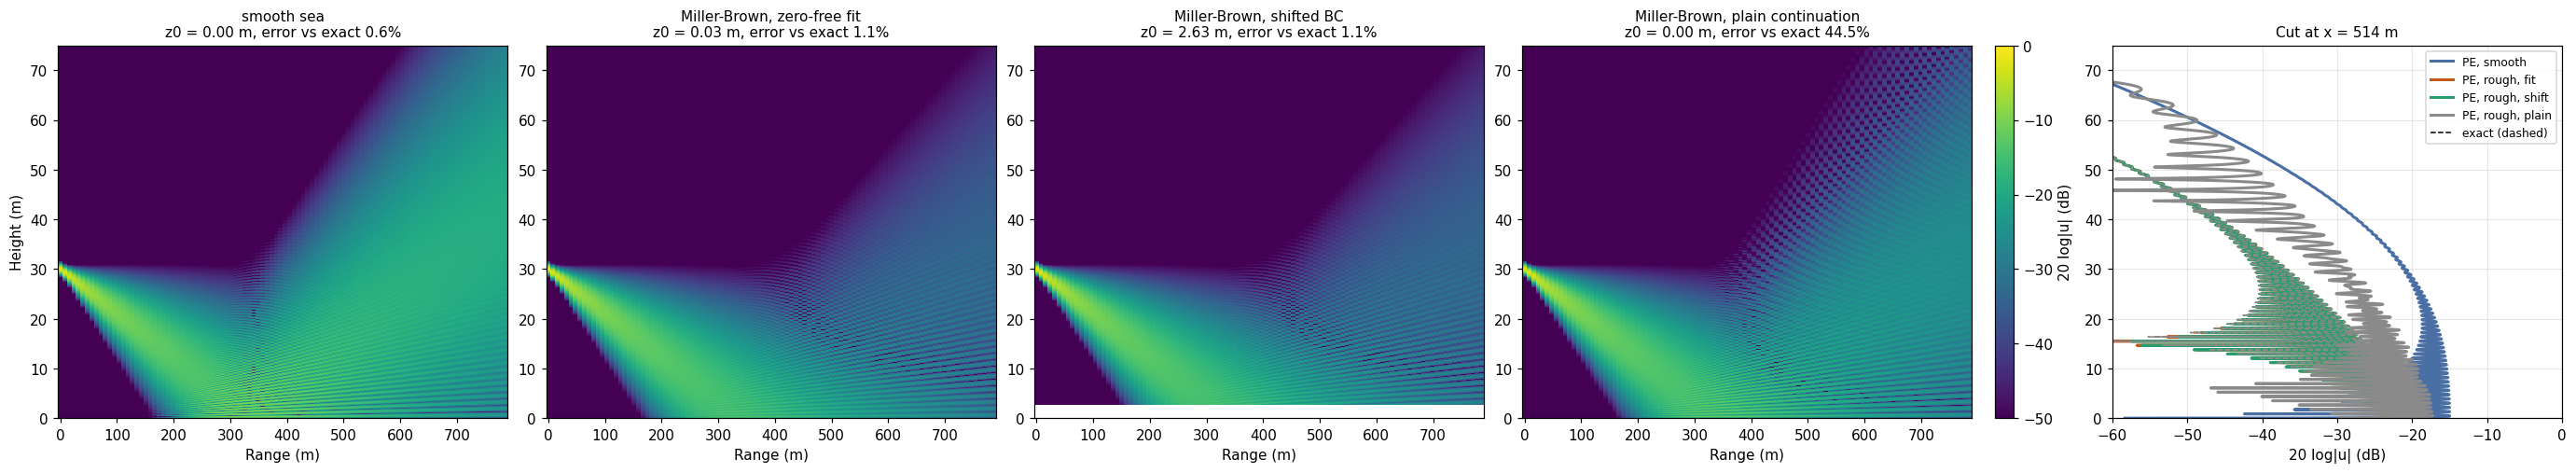
\includegraphics[width=\linewidth]{rough_sea_nlbc_demo.png}
  \caption{\SI{3}{GHz} H-pol beam at \ang{5} grazing over a sea with
  $\sigma=\SI{0.3}{m}$: smooth sea, zero-free fit, lifted reference plane, plain
  continuation, and a vertical cut through the reflected beam against the exact
  solution (dashed).}
  \label{fig:demo}
\end{figure}

\subsection{Long-range demonstration}
A \SI{20}{m} H-pol antenna with a \ang{2} beam radiates over \SI{60}{km} of sea
($\varepsilon=70$, \SI{4}{S/m}) at 1, 3 and \SI{10}{GHz}, for wind speeds of 0, 5, 10
and \SI{15}{m/s} and three refractivity profiles: standard atmosphere, a \SI{15}{m}
evaporation duct, and a surface-based duct with a \SI{30}{m} trapping layer at
\SI{100}{m}. All 36 cases are stable. Figures~\ref{fig:maps}--\ref{fig:excess} show
the results, and Table~\ref{tab:long} gives the roughness-induced loss.

\begin{table}[t]
  \centering
  \caption{Roughness-induced excess path loss (dB) at \SI{10}{m} height: mean over
  20--\SI{60}{km} / value at \SI{58}{km}, for wind speeds 5, 10 and \SI{15}{m/s}
  ($\sigma=0.13$, 0.51, \SI{1.15}{m}). Negative values beyond the horizon in the
  standard atmosphere are the Miller--Brown lateral wave (Section~\ref{sec:lateral}).}
  \label{tab:long}
  \begin{tabular}{llccc}
    \toprule
    Profile & Band & \SI{5}{m/s} & \SI{10}{m/s} & \SI{15}{m/s} \\
    \midrule
    Standard     & L & $+0.0/+0.0$ & $+0.2/+0.7$  & $+0.7/+3.7$ \\
                 & S & $+0.1/+0.2$ & $+1.0/+2.8$  & $+1.3/-8.7$ \\
                 & X & $-0.9/-7.0$ & $-4.0/-26.4$ & $-12.0/-39.7$ \\
    \midrule
    Evaporation  & L & $0.0/0.0$   & $0.0/0.0$    & $0.0/-0.1$ \\
    duct 15 m    & S & $0.0/0.0$   & $0.0/0.0$    & $+0.1/0.0$ \\
                 & X & $+0.2/+0.3$ & $+2.1/+2.6$  & $+4.5/+6.4$ \\
    \midrule
    Surface-based& L & $0.0/0.0$   & $+0.1/+0.1$  & $+0.1/+0.2$ \\
    duct         & S & $0.0/0.0$   & $0.0/+0.3$   & $+0.1/+1.1$ \\
                 & X & $0.0/+0.1$  & $+0.5/+1.8$  & $+0.8/+4.9$ \\
    \bottomrule
  \end{tabular}
\end{table}

\begin{figure}[p]
  \centering
  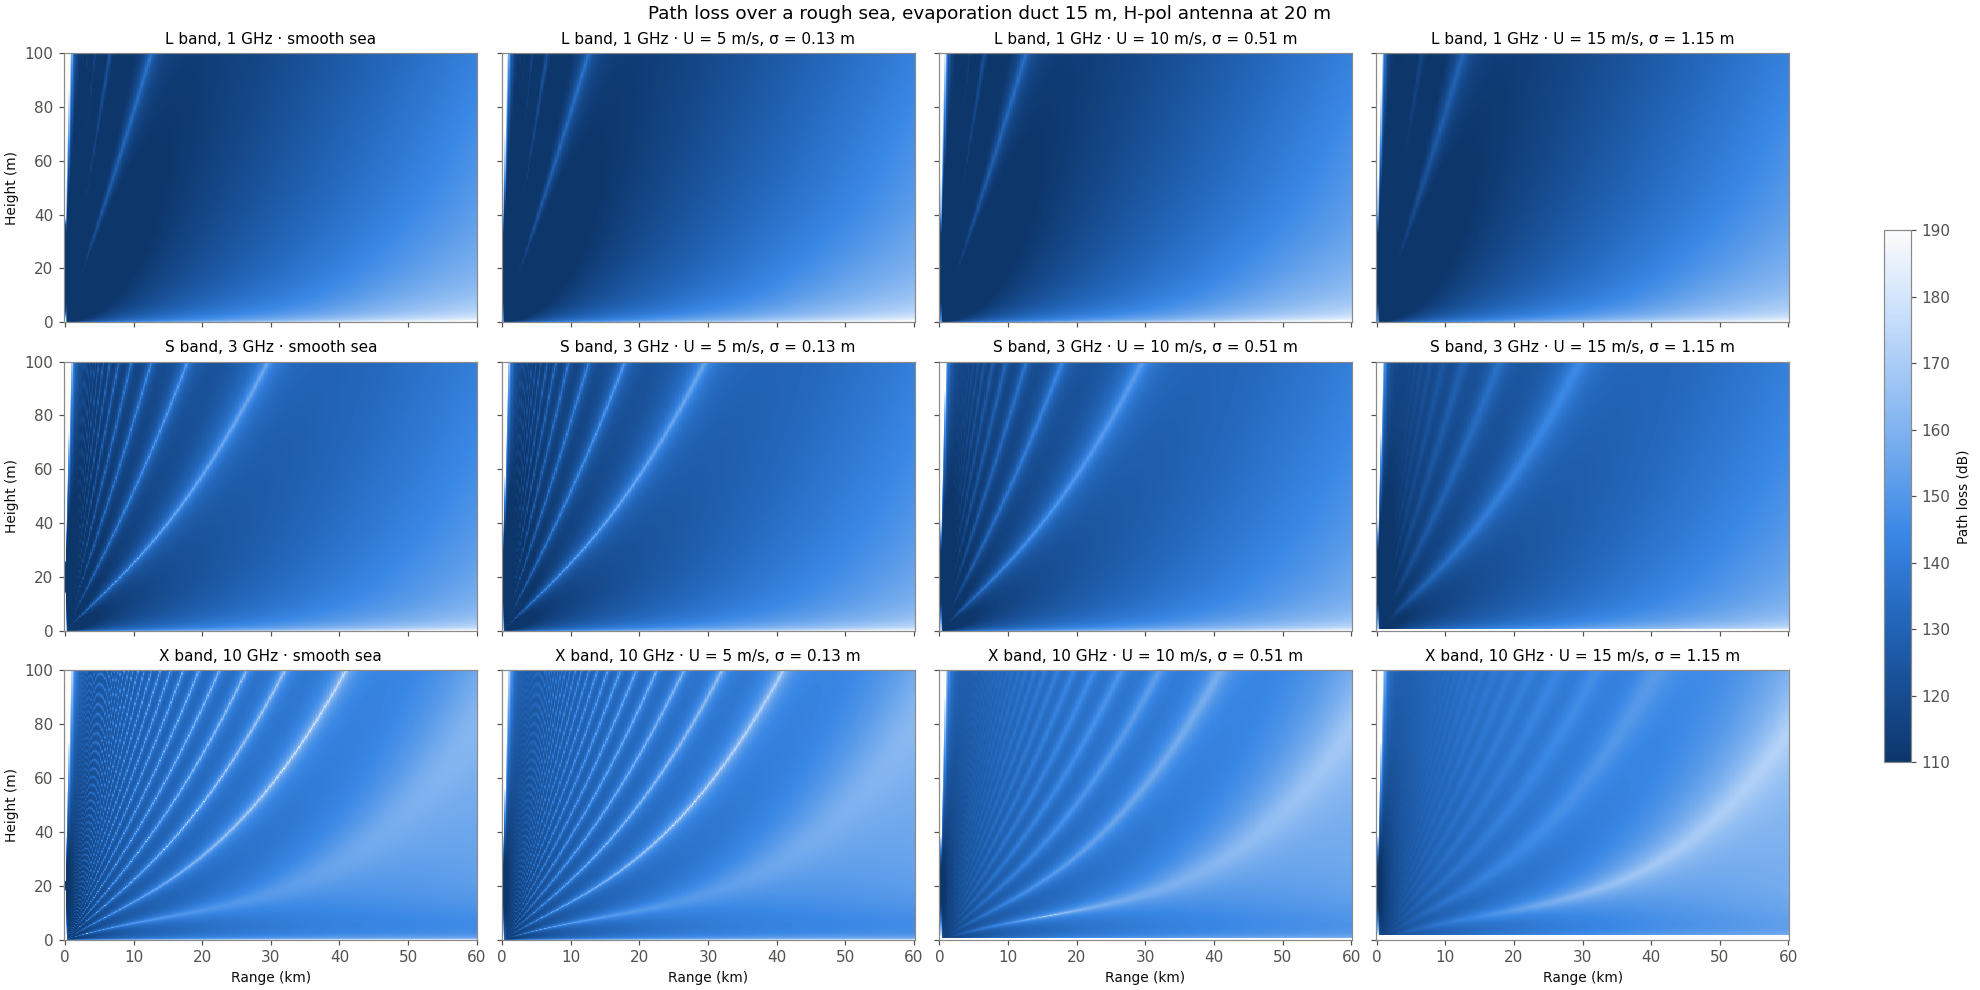
\includegraphics[width=\linewidth]{rough_sea_long_range_maps_evaporation.png}\\[2mm]
  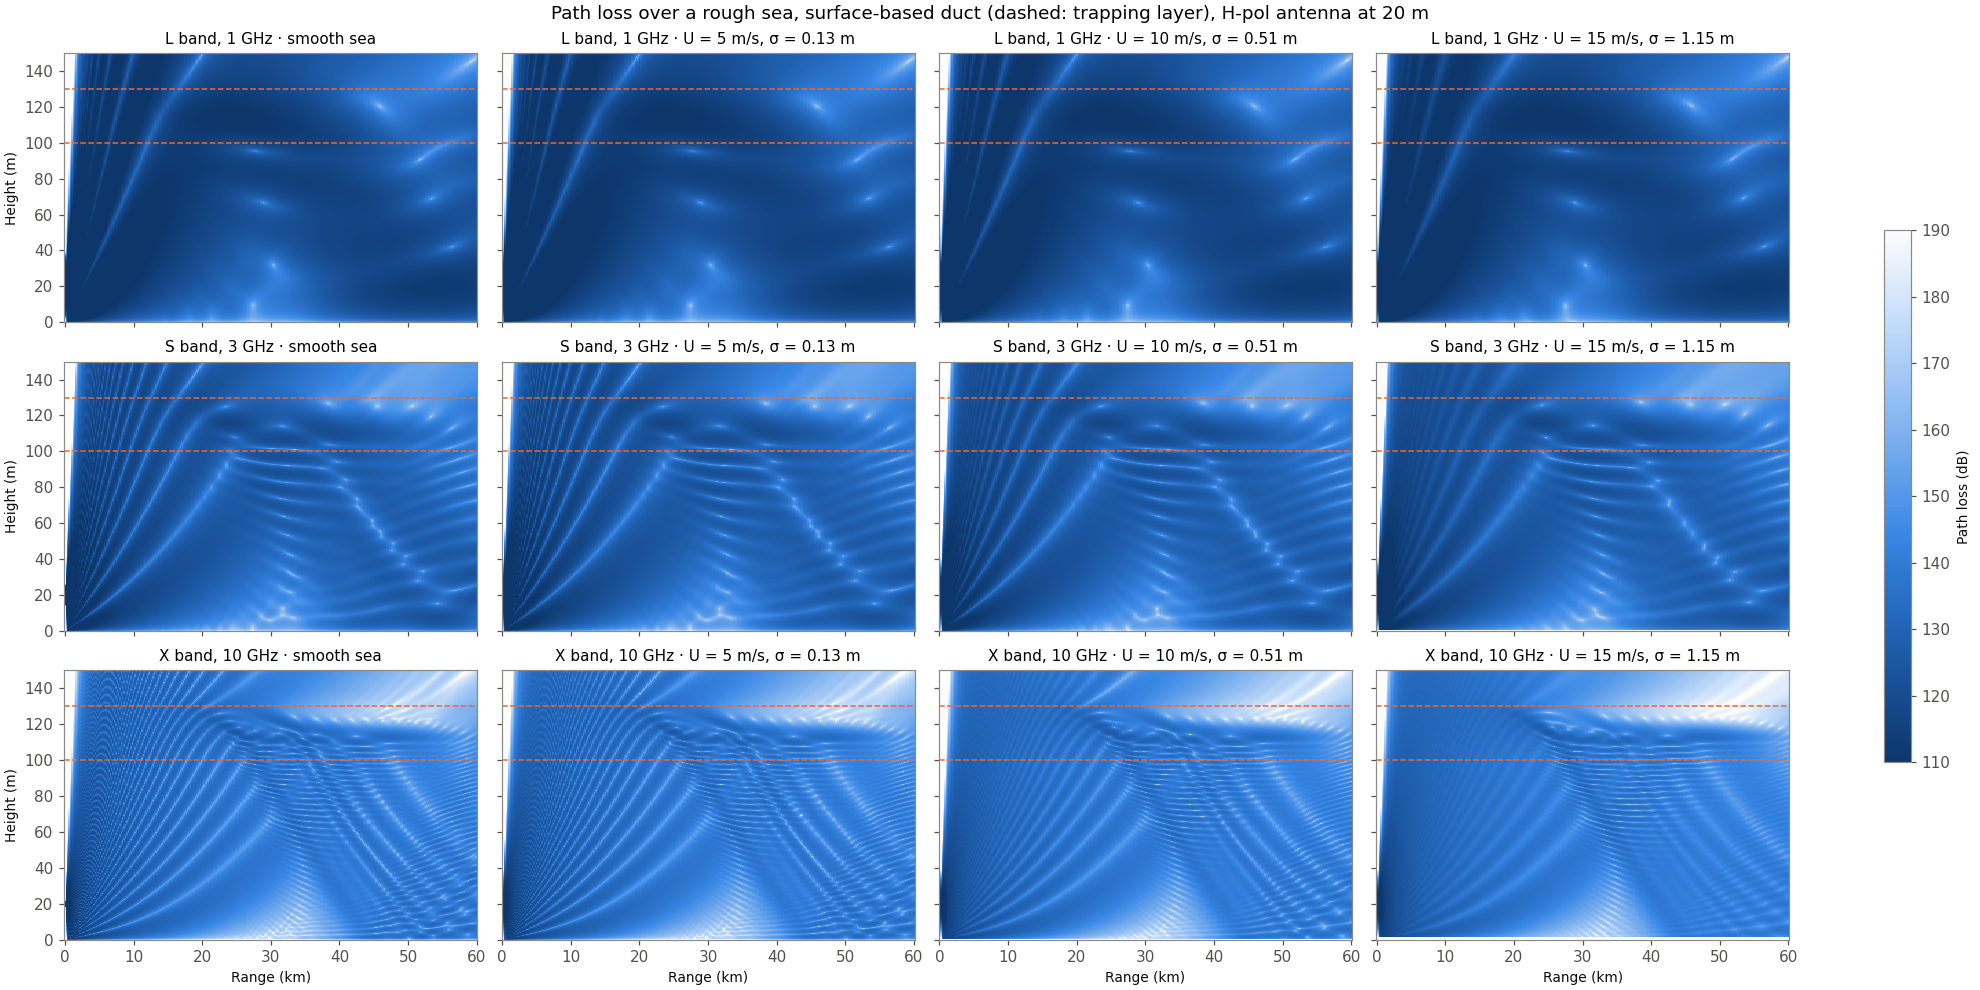
\includegraphics[width=\linewidth]{rough_sea_long_range_maps_surface.png}
  \caption{Path loss over a rough sea: \SI{15}{m} evaporation duct (top) and
  surface-based duct (bottom, dashed: trapping layer). Rows: L, S, X band;
  columns: smooth sea and 5, 10, \SI{15}{m/s}.}
  \label{fig:maps}
\end{figure}

\begin{figure}[t]
  \centering
  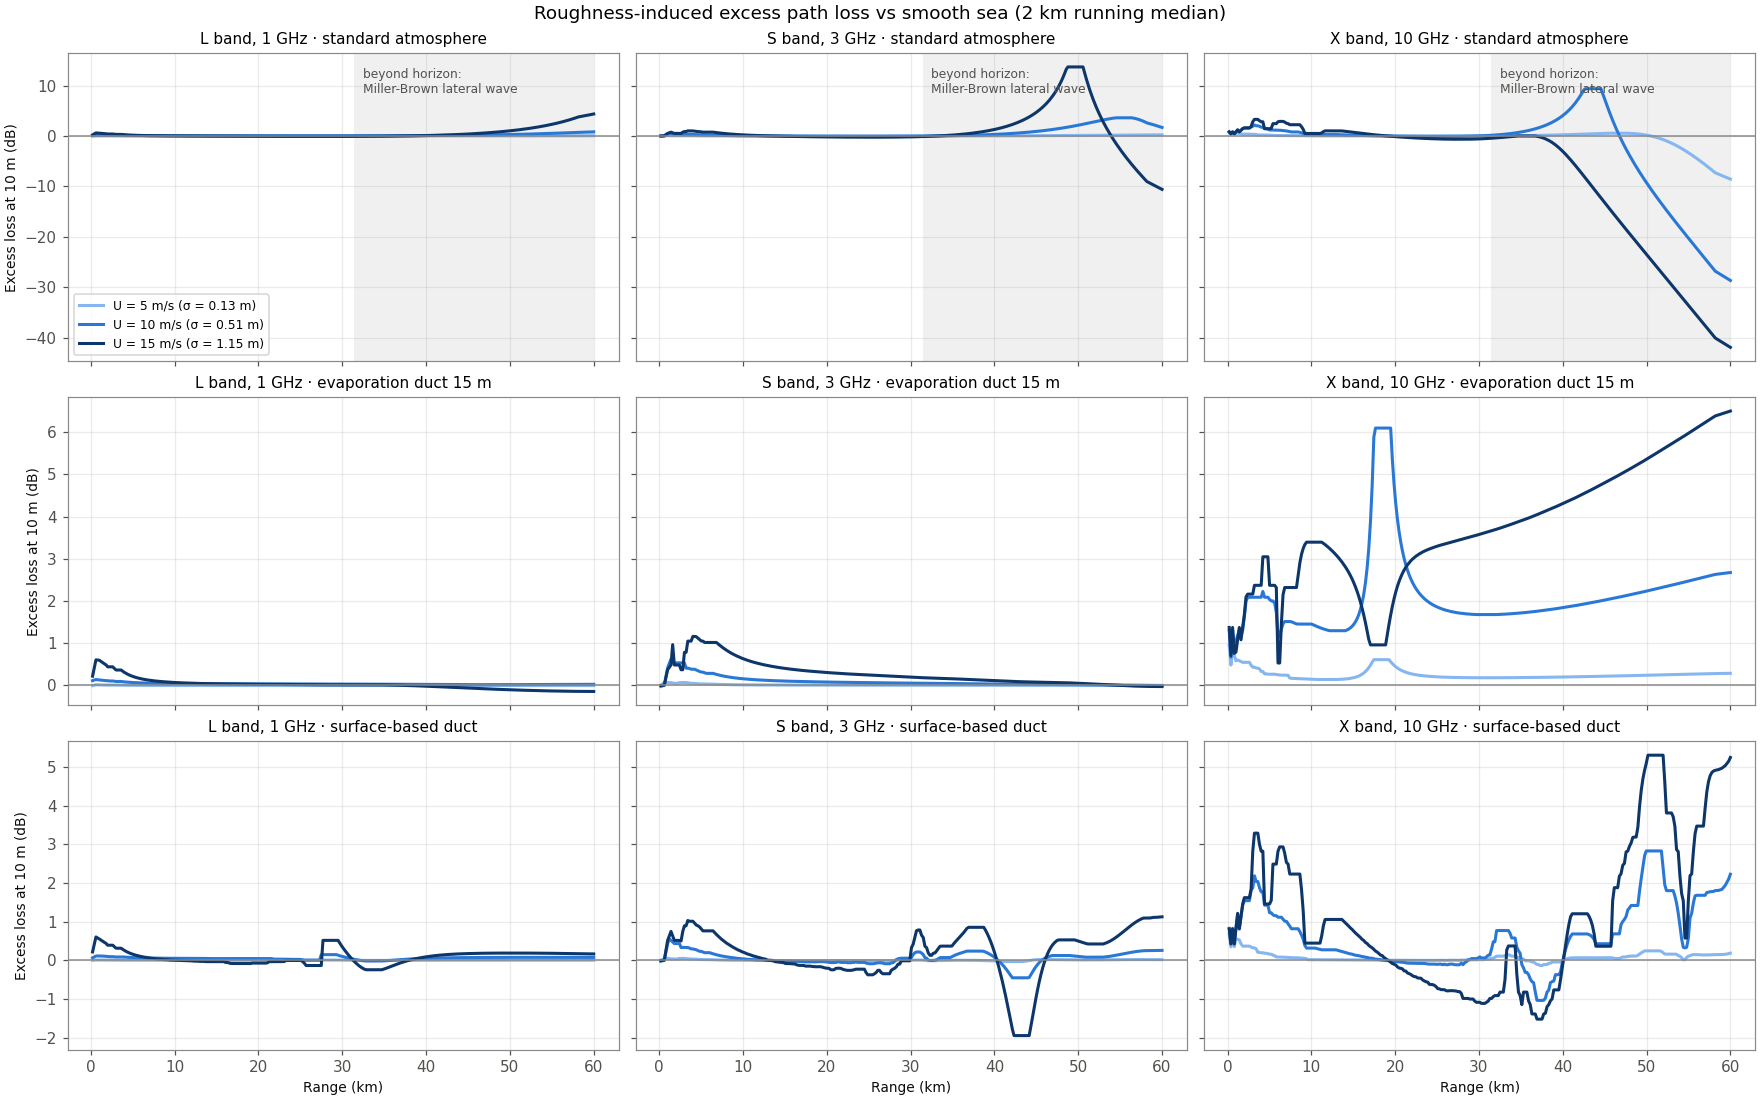
\includegraphics[width=\linewidth]{rough_sea_long_range_excess.png}
  \caption{Roughness-induced excess path loss at \SI{10}{m} height vs range
  (2\,km running median). Shaded: beyond the radio horizon in the standard
  atmosphere, where the Miller--Brown lateral wave dominates (Section~\ref{sec:lateral}).}
  \label{fig:excess}
\end{figure}

\paragraph{Discussion.}
In the evaporation duct at X band the roughness-induced loss grows steadily
with range, by about \SI{0.1}{dB/km} at \SI{15}{m/s}, reaching \SI{6.4}{dB} at
\SI{58}{km}. The ducted field is carried by the lowest trapped modes, which meet the
surface at about \ang{0.1}. There the Miller--Brown factor is 0.73 at \SI{15}{m/s},
i.e.\ \SI{-2.8}{dB} per bounce with a bounce every 17\,km or so: about
\SI{0.16}{dB/km}, the same order as the computed rate. At 60\,km the effect is
moderate; if the rate persists, it would reach 10--\SI{15}{dB} over 100--\SI{150}{km}. At S and L band roughness is negligible in the ducts, since
$k\sigma\sin\psi$ stays small at the grazing angles of the trapped energy. In the
surface-based duct, the energy trapped below the layer at \SI{100}{m} interacts with
the surface less often; roughness smooths the interference pattern below about
\SI{60}{m} at X band (Fig.~\ref{fig:maps}) and adds up to \SI{5}{dB} of loss. Within the
horizon in the standard atmosphere roughness changes the loss by less than
\SI{1}{dB}. Beyond the horizon the Miller--Brown lateral wave dominates. The fitted
coefficient needed lifts of 0--\SI{0.86}{m} in all cases except X band at
\SI{15}{m/s} in the ducts (\SI{1.72}{m}), against 15--\SI{78}{m} for the pure lift.
Section~\ref{sec:barrick} revisits the beyond-horizon cases with the constant grazing
impedance.

\paragraph{Computational cost.}
A rough-sea model requires a probe of the grid (no lower NLBC), the contour,
a few least-squares fits, and the lower NLBC. Builds take 10--\SI{65}{s} at L and S
band and about \SI{3}{min} at X band over \SI{60}{km} (five models in parallel on
20 cores). The constant grazing impedance builds about twice as fast at S band and
needs smaller lifts (none in the standard atmosphere at S band). When several models are
built in parallel processes, the BLAS threads of each process must be limited. With
four processes on 20 cores and default thread pools, OpenBLAS busy-waiting made the
fits about 20 times slower (1430\,s against 67\,s per model).

%=====================================================================
\section{Conclusions}
The discrete NLBC handles a rough sea once the reflection coefficient is given a
suitable continuation. The plain continuation of the Miller--Brown factor is
unstable, and no bounded continuation can be exact near grazing. A zero-free
fitted coefficient $1+\Rt=(1+R_f)e^K$, with at most a small lift of the reference
plane, reproduces Miller--Brown to about 1\,\%. Its stability on long-range problems
requires, beyond zero-freeness, passivity for propagating waves and in the trapping
range of the atmosphere, and accuracy on the wavenumbers of range-decaying modes.
In ducts the expected roughness-induced attenuation that grows with range is
obtained at X band, and roughness is negligible at L band. Beyond the horizon
Miller--Brown raises the field substantially; the comparison with an independent
modal and branch-cut solution identifies this as the lateral wave of the model at
grazing incidence, where its effective impedance behaves like $1/\kz$. This
contradicts the constant grazing impedance of rough surfaces \cite{barrick1998}. A
blend that freezes the Miller--Brown roughness admittance below the Rayleigh angle
removes the lateral wave, and with the fit matched to first order at grazing the PE
reproduces the creeping modes of the resulting impedance to \SI{0.01}{dB/km}. The
value of the grazing impedance remains to be calibrated against rigorous solutions
over sea surfaces generated from wave spectra; the boundary condition accepts any
such calibrated coefficient.

\begin{thebibliography}{99}
\bibitem{lytaev2022} M.~S. Lytaev, ``Fresnel reflection modeling within the
  higher-order parabolic equation and discrete nonlocal boundary conditions,''
  in \emph{IEEE Radar Conference}, 2022.
\bibitem{mbv1984} A.~R. Miller, R.~M. Brown, and E.~Vegh, ``New derivation for the
  rough-surface reflection coefficient and for the distribution of sea-wave
  elevations,'' \emph{IEE Proc. H}, vol.~131, no.~2, pp.~114--116, 1984.
\bibitem{ament1953} W.~S. Ament, ``Toward a theory of reflection by a rough
  surface,'' \emph{Proc. IRE}, vol.~41, no.~1, pp.~142--146, 1953.
\bibitem{levy2000} M.~F. Levy, \emph{Parabolic Equation Methods for Electromagnetic
  Wave Propagation}. London: IEE, 2000.
\bibitem{collins1993} M.~D. Collins, ``A split-step Pad\'e solution for the parabolic
  equation method,'' \emph{J. Acoust. Soc. Am.}, vol.~93, no.~4, pp.~1736--1742, 1993.
\bibitem{brubeck2021} P.~D. Brubeck, Y.~Nakatsukasa, and L.~N. Trefethen,
  ``Vandermonde with Arnoldi,'' \emph{SIAM Review}, vol.~63, no.~2, pp.~405--415, 2021.
\bibitem{freund2006} D.~E. Freund, N.~E. Woods, H.-C. Ku, and R.~S. Awadallah,
  ``Forward radar propagation over a rough sea surface: a numerical assessment of
  the Miller--Brown approximation using a horizontally polarized 3-GHz line
  source,'' \emph{IEEE Trans. Antennas Propag.}, vol.~54, no.~4, pp.~1292--1304, 2006.
\bibitem{barrick1998} D.~E. Barrick, ``Grazing behavior of scatter and propagation
  above any rough surface,'' \emph{IEEE Trans. Antennas Propag.}, vol.~46, no.~1,
  pp.~73--83, 1998.
\bibitem{barrick1971} D.~E. Barrick, ``Theory of HF and VHF propagation across the
  rough sea, 1: The effective surface impedance for a slightly rough highly
  conducting medium at grazing incidence,'' \emph{Radio Sci.}, vol.~6, no.~5,
  pp.~517--526, 1971.
\bibitem{ishimaru2000} A.~Ishimaru, J.~D. Rockway, Y.~Kuga, and S.-W. Lee,
  ``Sommerfeld and Zenneck wave propagation for a finitely conducting
  one-dimensional rough surface,'' \emph{IEEE Trans. Antennas Propag.}, vol.~48,
  no.~9, pp.~1475--1484, 2000.
\bibitem{lai2004} Z.~Lai \emph{et al.}, ``Equivalent impedance of a large rough
  surface at low grazing angles,'' in \emph{IEEE Antennas Propag. Soc. Symp.}, 2004.
\bibitem{fabbro2006} V.~Fabbro, C.~Bourlier, and P.~F. Combes, ``Forward propagation
  modeling above Gaussian rough surfaces by the parabolic wave equation:
  introduction of the shadowing effect,'' \emph{Prog. Electromagn. Res.}, vol.~58,
  pp.~243--269, 2006.
\bibitem{song2024} G.~Song \emph{et al.}, ``Effect of rough sea surface on
  electromagnetic wave propagation in evaporation duct environment,'' in
  \emph{Int. Symp. Antennas, Propag. EM Theory (ISAPE)}, 2024.
\bibitem{zhao2025} P.-C. Zhao \emph{et al.}, ``A fast method for predicting radio
  waves propagation over rough sea surfaces,'' \emph{IEEE Antennas Wireless Propag.
  Lett.}, 2025.
\bibitem{voronovich1994} A.~G. Voronovich, \emph{Wave Scattering from Rough
  Surfaces}. Berlin: Springer, 1994.
\bibitem{pm1964} W.~J. Pierson and L.~Moskowitz, ``A proposed spectral form for fully
  developed wind seas based on the similarity theory of S.~A. Kitaigorodskii,''
  \emph{J. Geophys. Res.}, vol.~69, no.~24, pp.~5181--5190, 1964.
\bibitem{hasselmann1973} K.~Hasselmann \emph{et al.}, ``Measurements of wind-wave
  growth and swell decay during the Joint North Sea Wave Project (JONSWAP),''
  \emph{Dtsch. Hydrogr. Z.}, Suppl.~A8, no.~12, 1973.
\bibitem{elfouhaily1997} T.~Elfouhaily, B.~Chapron, K.~Katsaros, and
  D.~Vandemark, ``A unified directional spectrum for long and short wind-driven
  waves,'' \emph{J. Geophys. Res.}, vol.~102, no.~C7, pp.~15781--15796, 1997.
\bibitem{gao2019} Y.~Gao \emph{et al.}, ``Parabolic equation modeling of
  electromagnetic wave propagation over rough sea surfaces,'' \emph{Sensors},
  vol.~19, no.~5, 1252, 2019.
\bibitem{guo2020} Q.~Guo \emph{et al.}, ``Two-way parabolic equation method for radio
  propagation over rough sea surface,'' \emph{IEEE Trans. Antennas Propag.},
  vol.~68, p.~4839, 2020.
\bibitem{ji2025} H.~Ji \emph{et al.}, ``Numerical modeling of electromagnetic wave
  propagation in spatially-varying evaporation duct conditions via 3D parabolic
  equation method,'' \emph{Front. Mar. Sci.}, 2025.
\bibitem{bonnafont2024} T.~Bonnafont \emph{et al.}, ``Long-range electromagnetic
  propagation above a polluted sea surface: hybrid modeling,'' \emph{IEEE Geosci.
  Remote Sens. Lett.}, 2024.
\end{thebibliography}

\end{document}
